\documentclass[a4paper,12pt]{article}
\usepackage{lmodern}
\usepackage{amssymb,amsmath}
\usepackage{ifxetex,ifluatex}
\usepackage{fixltx2e} % provides \textsubscript
\ifnum 0\ifxetex 1\fi\ifluatex 1\fi=0 % if pdftex
  \usepackage[T1]{fontenc}
  \usepackage[utf8]{inputenc}
\else % if luatex or xelatex
  \ifxetex
    \usepackage{mathspec}
  \else
    \usepackage{fontspec}
  \fi
  \defaultfontfeatures{Ligatures=TeX,Scale=MatchLowercase}
\fi
% use upquote if available, for straight quotes in verbatim environments
\IfFileExists{upquote.sty}{\usepackage{upquote}}{}
% use microtype if available
\IfFileExists{microtype.sty}{%
\usepackage{microtype}
\UseMicrotypeSet[protrusion]{basicmath} % disable protrusion for tt fonts
}{}
\usepackage{hyperref}
\hypersetup{unicode=true,
            pdfborder={0 0 0},
            breaklinks=true}
\urlstyle{same}  % don't use monospace font for urls
\usepackage{graphicx,grffile}
\makeatletter
\def\maxwidth{\ifdim\Gin@nat@width>\linewidth\linewidth\else\Gin@nat@width\fi}
\def\maxheight{\ifdim\Gin@nat@height>\textheight\textheight\else\Gin@nat@height\fi}
\makeatother
% Scale images if necessary, so that they will not overflow the page
% margins by default, and it is still possible to overwrite the defaults
% using explicit options in \includegraphics[scale=0.5][Gin}{width=\maxwidth,height=\maxheight,keepaspectratio}
% Make links footnotes instead of hotlinks:
\renewcommand{\href}[2]{#2\footnote{See \texttt{\url{#1}}}}
\setlength{\emergencystretch}{3em}  % prevent overfull lines
\providecommand{\tightlist}{%
  \setlength{\itemsep}{0pt}\setlength{\parskip}{0pt}}
\setcounter{secnumdepth}{5}
% Redefines (sub)paragraphs to behave more like sections
\ifx\paragraph\undefined\else
\let\oldparagraph\paragraph
\renewcommand{\paragraph}[1]{\oldparagraph{#1}\mbox{}}
\fi
\ifx\subparagraph\undefined\else
\let\oldsubparagraph\subparagraph
\renewcommand{\subparagraph}[1]{\oldsubparagraph{#1}\mbox{}}
\fi

\date{}


%
% Line Spread, Page Markings & Hyperlinked Documents
%
\linespread{1.3}
% Margin:
\usepackage[top=1.5in, bottom=1.5in, right=1in, left=1in]{geometry}

% To silence too small headheight warning
\setlength{\headheight}{15pt}

% Header & Footer:
\usepackage{fancyhdr}
\pagestyle{fancy}
\fancyhf{} % Clear all header and footer fields
\fancyhead[LO,RE]{Helpdesk Ticketing System\\{\vspace{-2pt}\scriptsize Semester 1}}
\fancyhead[LE,RO]{\leftmark\\{\vspace{-4pt}\scriptsize SWE40001 Software Engineering Project}}
\fancyfoot[LE,RO]{\thepage\ifodd\value{page}\else\hfill\fi}
\usepackage{float}

\begin{document}

{
\setcounter{tocdepth}{3}
\tableofcontents
\listoffigures
}
\newpage
\section{Invision}\label{invision}

Prototypes have been designed using
\href{http://invisionapp.com}{InVision}

\section{iOS Prototype}\label{ios-prototype}

The iOS prototype is hosted at \texttt{\url{http://invis.io/4S76XFOKB}}.

\subsection{Tutor Queue}\label{tutor-queue}

\begin{figure}[p]
\centering
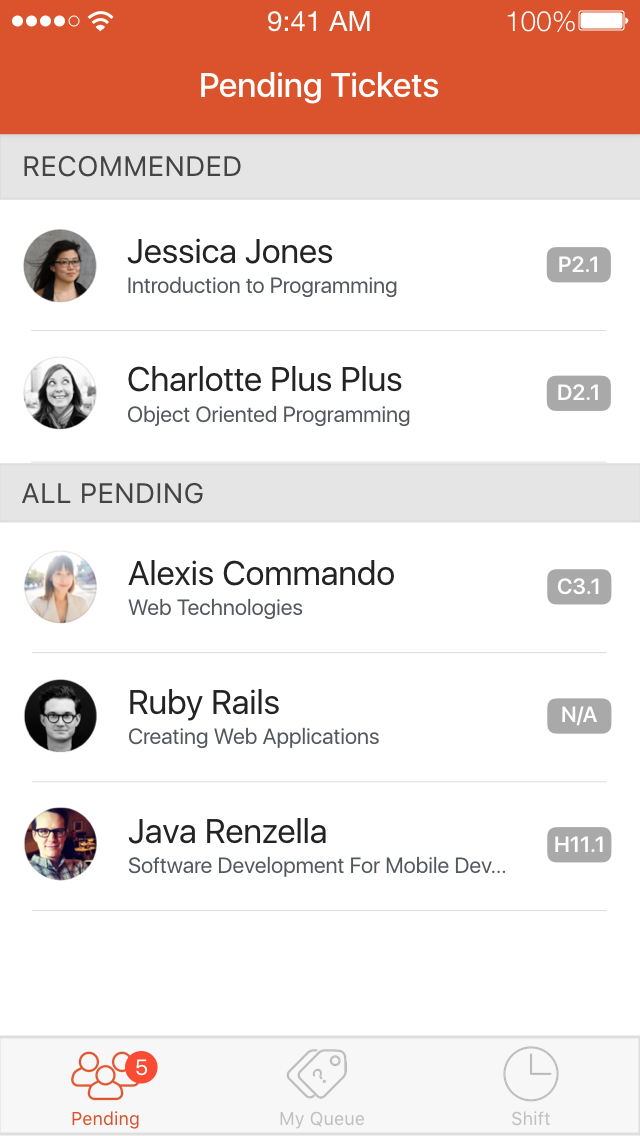
\includegraphics[scale=0.5]{46d5415602.png}
\caption{Global Queue}
\label{1}
\end{figure}

The global queue (Figure~\ref{1}) is shown when there are pending tickets. It is
separated between recommended and all pending students. Recommended
students show students who need help with subjects which the tutor
teaches. Badges on the side show the task abbreviation which students
need help with, if applicable.

Tutors can accept or defer tickets directly from their global queue, as shown
in Figure~\ref{2}.

The empty tutor queue is the queue when the ticket is empty. This means
there are no tickets in the tutor's local queue, meaning the tutor is
not currently helping any students. Figure~\ref{3} shows this, whereas
Figure~\ref{4} shows a queue with more students being helped by the tutor.

A tutor may choose to postpone a student directly from their queue (Figure~\ref{5}).
If a tutor skips the first student at the top of the list, the student
who has been seen the longest time ago or has never been seen at all,
then the app warns them. This is shown in the alert under Figure~\ref{6}.



\begin{figure}[p]
\centering
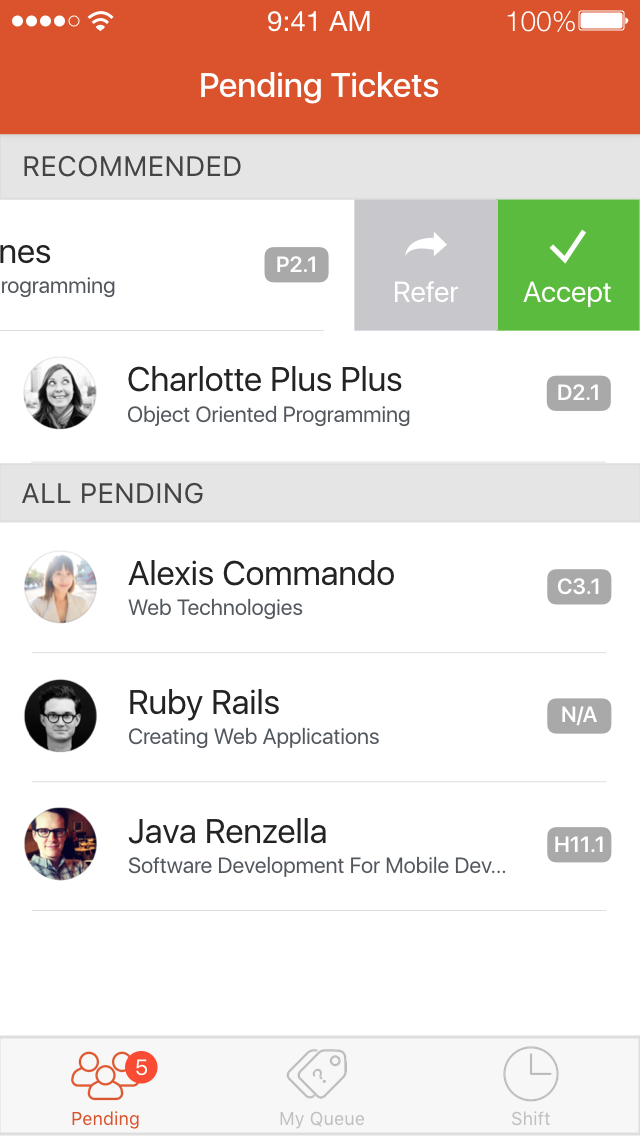
\includegraphics[scale=0.5]{c1f0491270.png}
\caption{Accept or Defer directly from the queue}
\label{2}
\end{figure}

\begin{figure}[p]
\centering
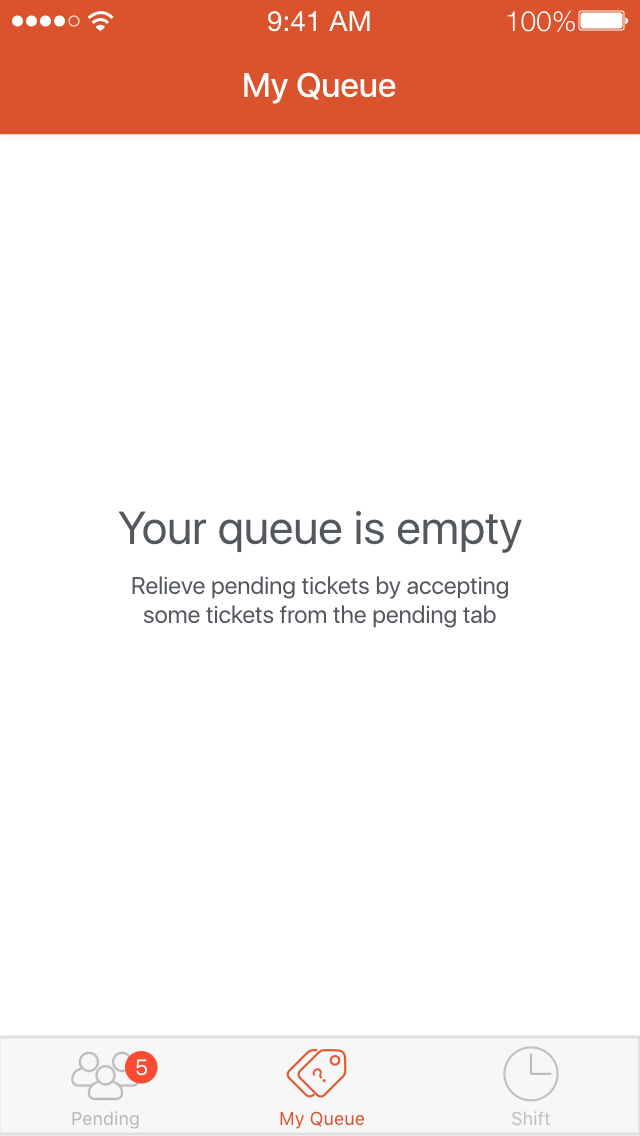
\includegraphics[scale=0.5]{4b296a8a4e.png}
\caption{Empty Tutor Queue}
\label{3}
\end{figure}

\begin{figure}[p]
\centering
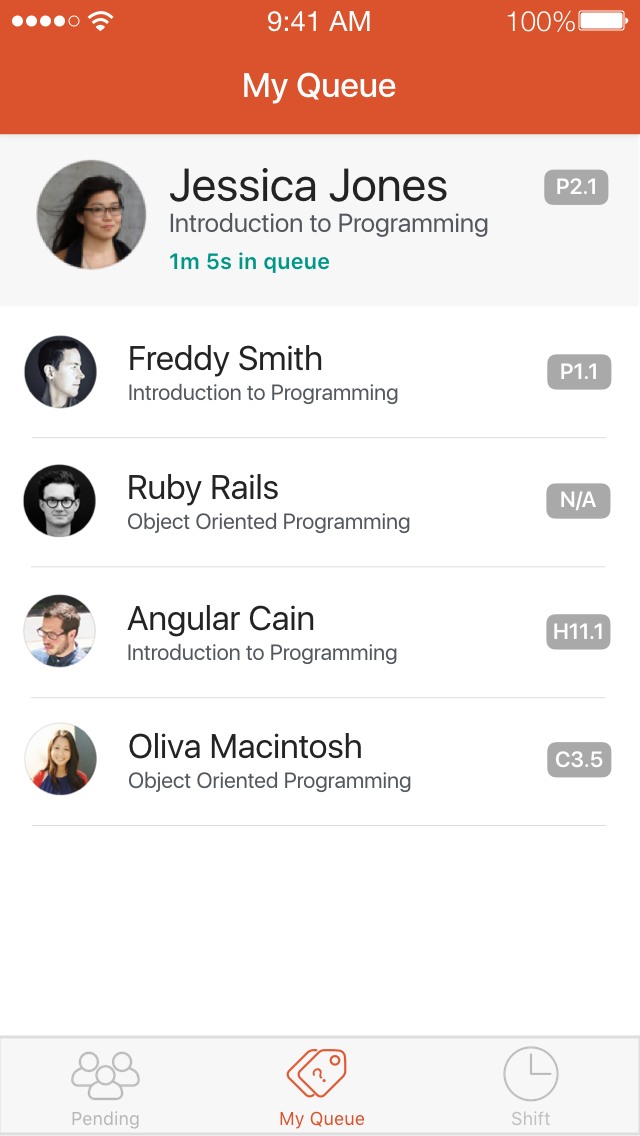
\includegraphics[scale=0.5]{2db52dc2d3.png}
\caption{Full Queue}
\label{4}
\end{figure}

\begin{figure}[p]
\centering
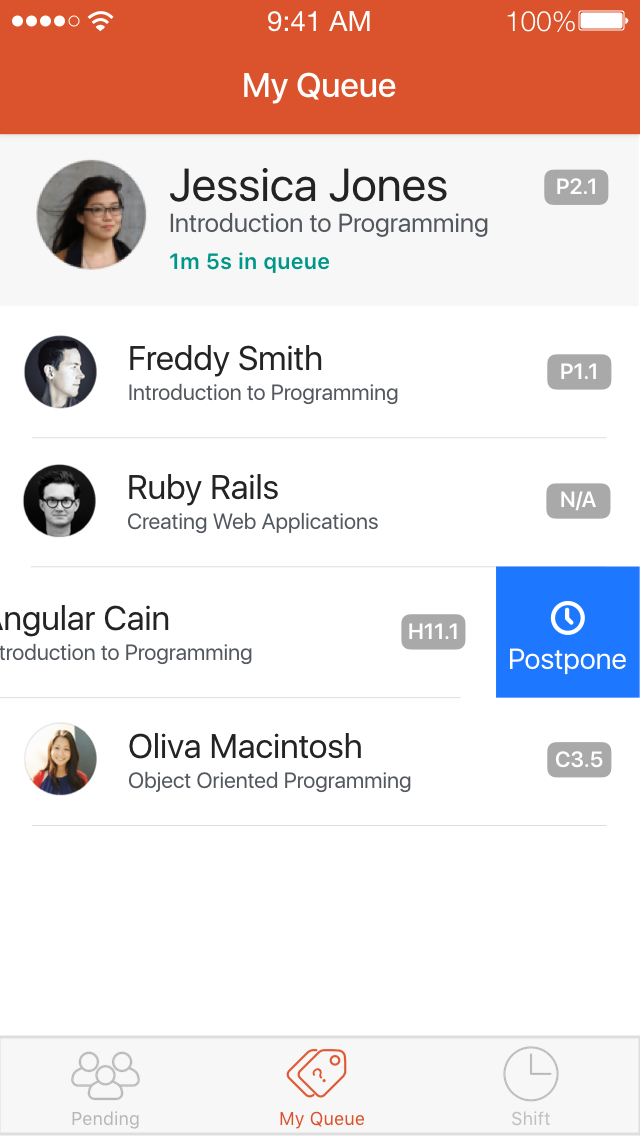
\includegraphics[scale=0.5]{4a2957343a.png}
\caption{Postpone Student Directly from the Queue}
\label{5}
\end{figure}

\begin{figure}[p]
\centering
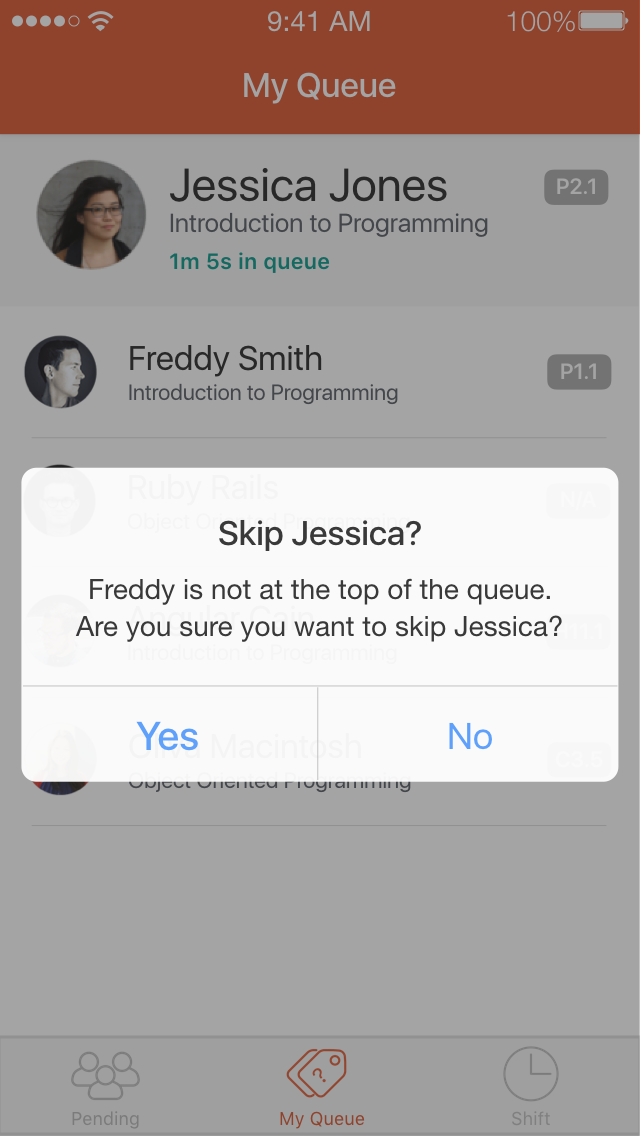
\includegraphics[scale=0.5]{59e78e9997.png}
\caption{Skip First Student Warning}
\label{6}
\end{figure}


\subsection{Ticket View}\label{ticket-view}

Tapping a ticket shows the details for the ticket. The same is shown for
both the global and tutor queue, however the primary actions differ. This is
shown under Figure~\ref{7}

When viewing a ticket from the tutor queue (Figure~\ref{8}), the ticket can be marked as
resolved or deferred (i.e., ``Come Back Later''). When the ticket is
viewed from the global queue, it can be taken aboard by the tutor
(accept ticket) or referred to another tutor.

Referring the ticket to another tutor shows tutors who are currently
working at the helpdesk and adds their ticket to their queue. This workflow
is illustrated under Figure~\ref{9}.

\begin{figure}[p]
\centering
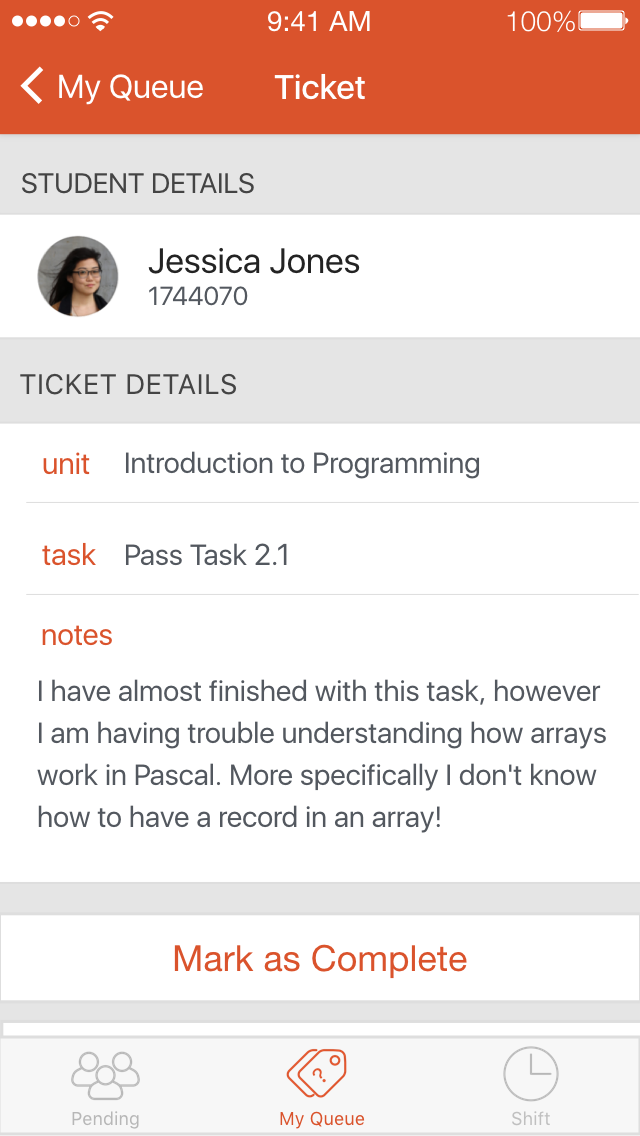
\includegraphics[scale=0.5]{35ca916310.png}
\caption{Tapping a student from the tutor queue}
\label{7}
\end{figure}



\begin{figure}[p]
\centering
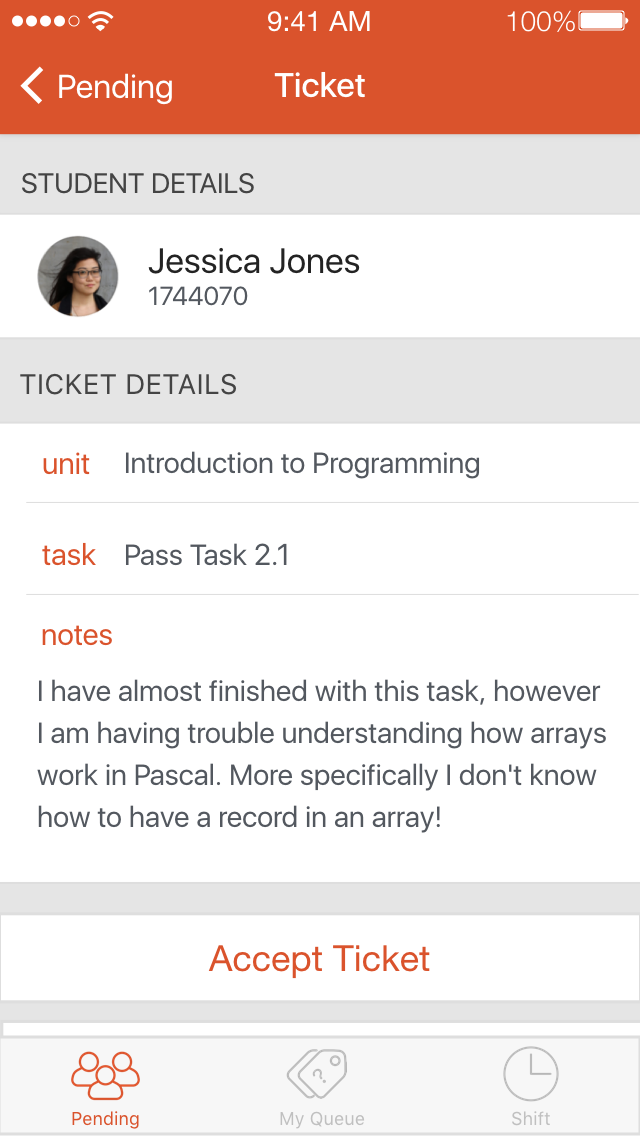
\includegraphics[scale=0.5]{72ea88c68f.png}
\caption{Tapping a Student from the global queue}
\label{8}
\end{figure}



\begin{figure}[p]
\centering
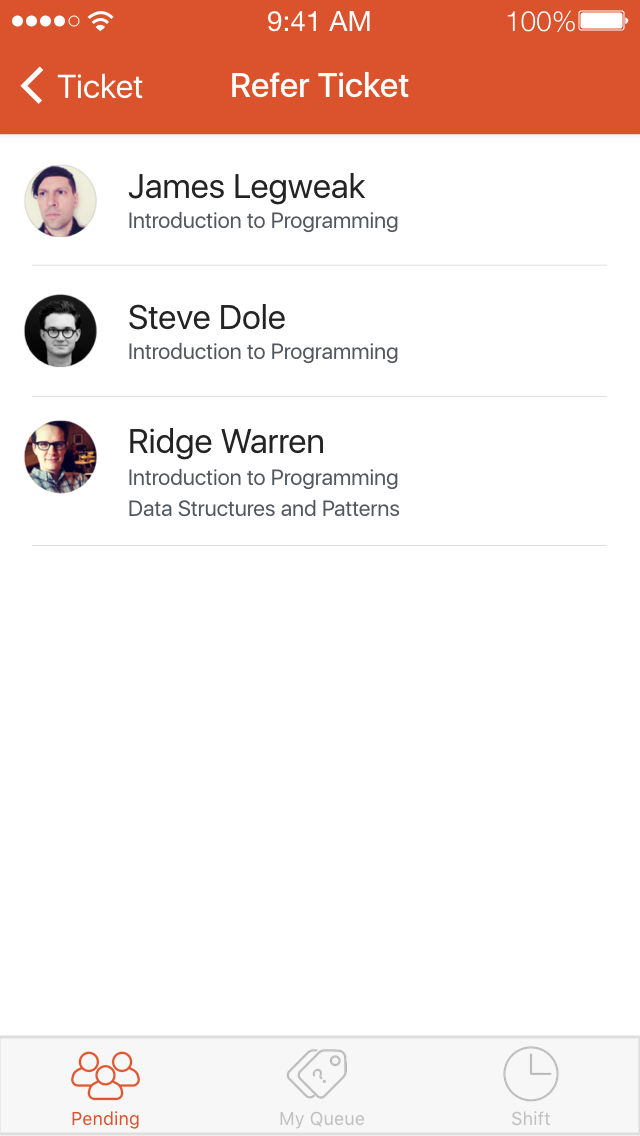
\includegraphics[scale=0.5]{91475c5923.png}
\caption{Referring a student to another tutor}
\label{9}
\end{figure}



\subsection{Push Notifications}\label{push-notifications}

Approaching the helpdesk connects to the BLE-enabled device at the
helpedesk and prompts them to clock on. When leaving the helpdesk, a push notification will warn them that they
are out of range and thus have clocked off.

Figures~\ref{10} and \ref{11} show this in more detail.

\begin{figure}[p]
\centering
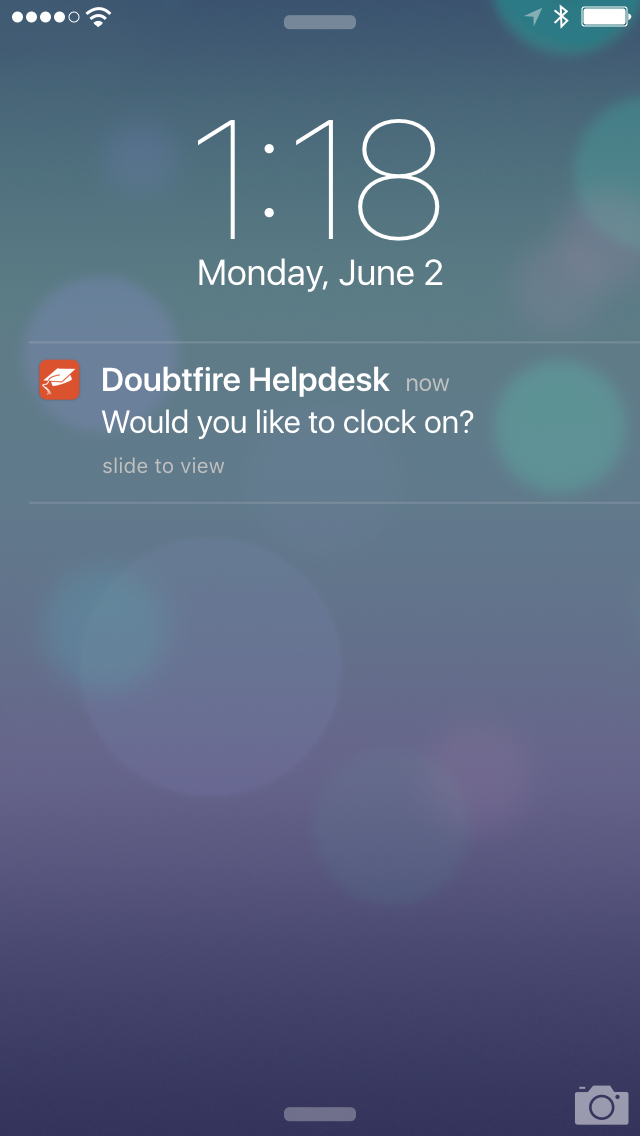
\includegraphics[scale=0.5]{30a3aff891.png}
\caption{Push Notification - Clock On}
\label{10}
\end{figure}



\begin{figure}[p]
\centering
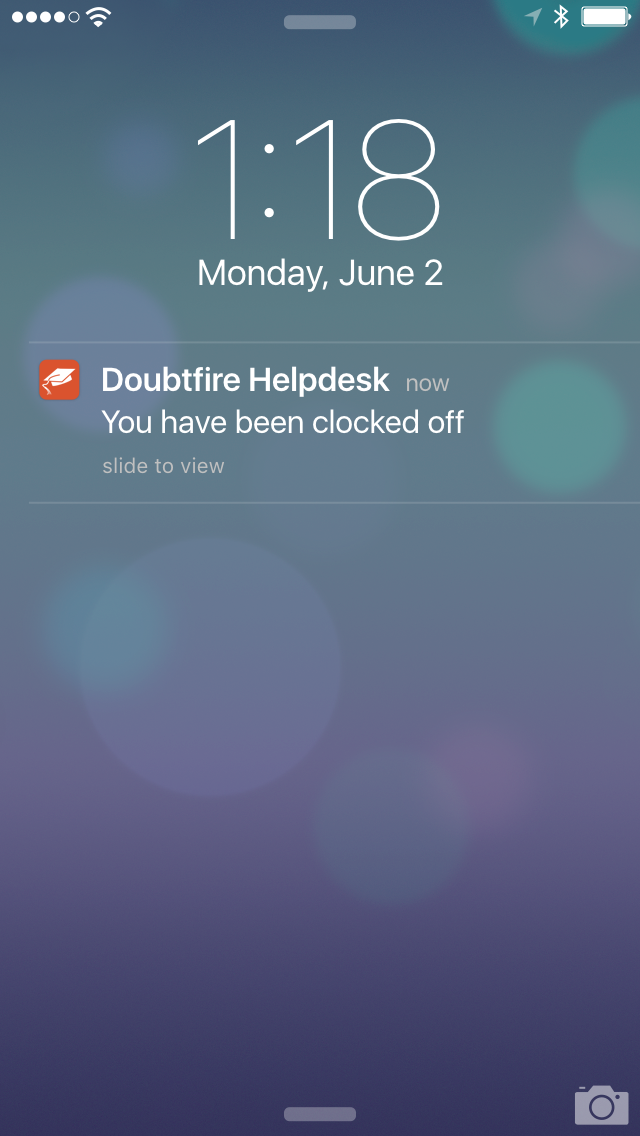
\includegraphics[scale=0.5]{7aeaf77695.png}
\caption{Push Notification - Clock Off}
\label{11}
\end{figure}



\subsection{Miscellaneous}\label{miscellaneous}

A basic sign in screen will use standard Doubtfire authentication,
i.e., SIMS. This is shown under the login view depicted in Figure~\ref{12}.

The about screen will show basic details, such as the Open-Source
license, as illustrated in Figure \ref{13}.

When bluetooth is disabled, a warning will be shown, preventing tutors to
continue using the app (Figure\ref{14}).

When a tutor disables auto-clock-on, then they can manually clock on by
this screen. This is shown in Figure~\ref{15}.

The shift tab shows details about the tutor's current shift (Figure~\ref{16}).
From the shift tab, a tutor can manually clock off (Figure~\ref{17}).

\section{Android Prototype}\label{android-prototype}

The Android prototype is hosted at \texttt{\url{http://invis.io/YF6Z1WRBM}}. It
follows the same workflow as the iOS app, except with Android-specific user
design paradigms.

\begin{figure}[p]
\centering
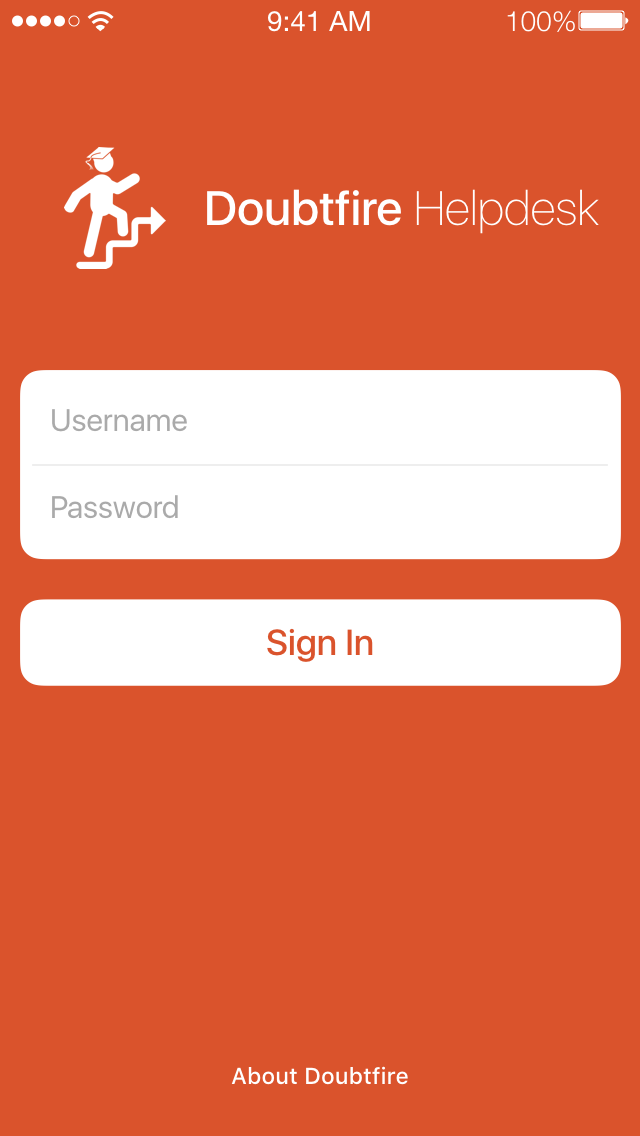
\includegraphics[scale=0.5]{5b7845cea9.png}
\caption{Sign In}
\label{12}
\end{figure}

\begin{figure}[p]
\centering
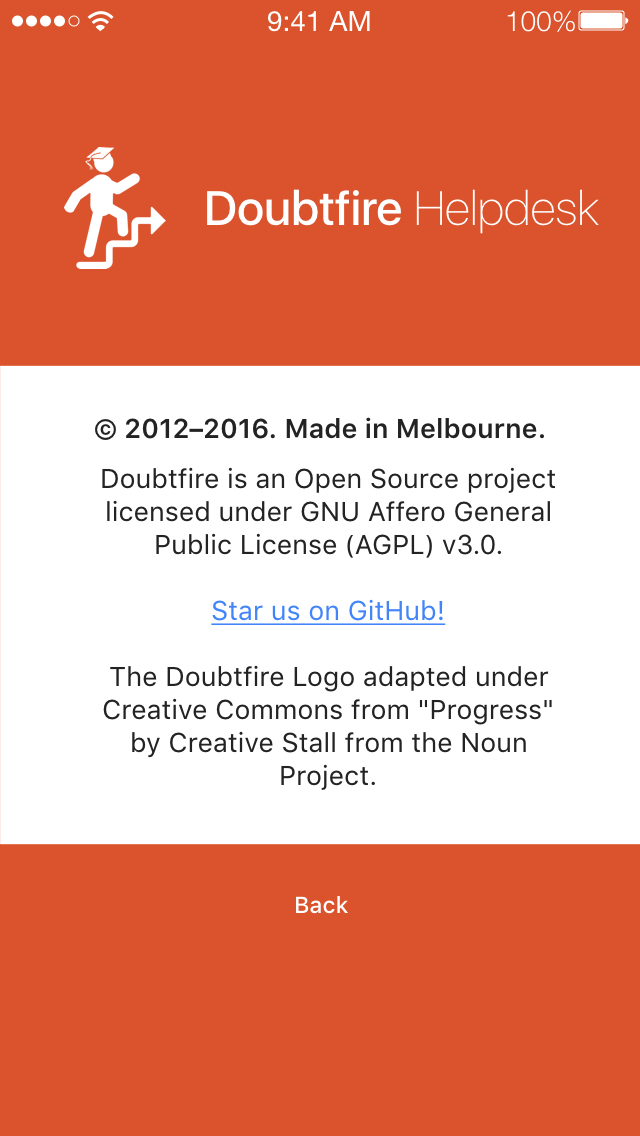
\includegraphics[scale=0.5]{64d7842b85.png}
\caption{About Doubtfire App}
\label{13}
\end{figure}


\begin{figure}[p]
\centering
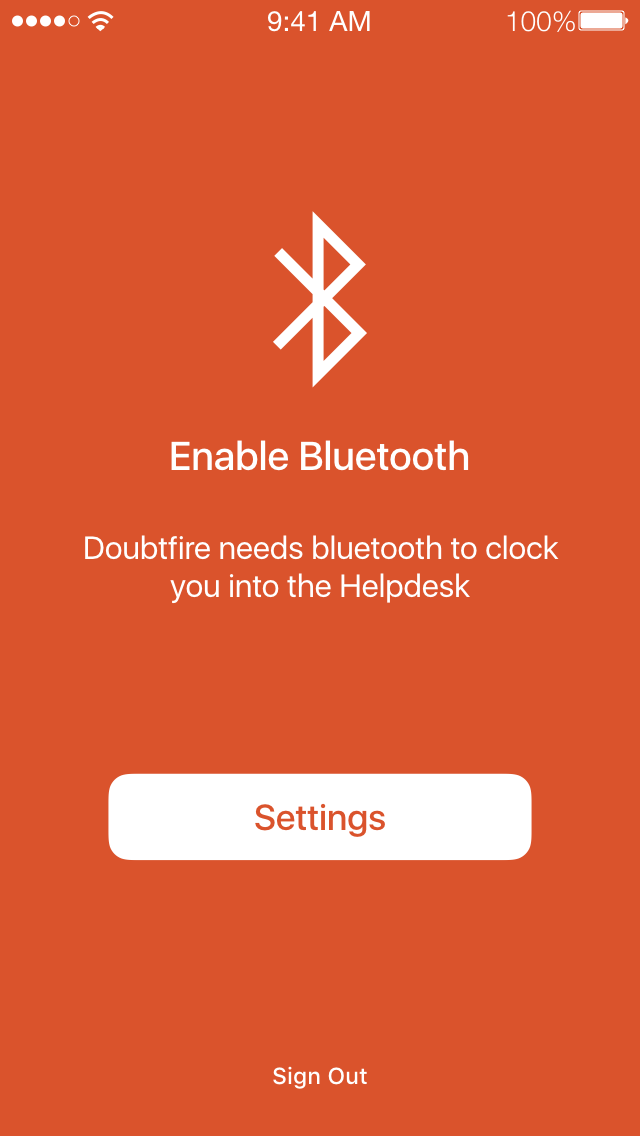
\includegraphics[scale=0.5]{f654931210.png}
\caption{Enable Bluetooth}
\label{14}
\end{figure}



\begin{figure}[p]
\centering
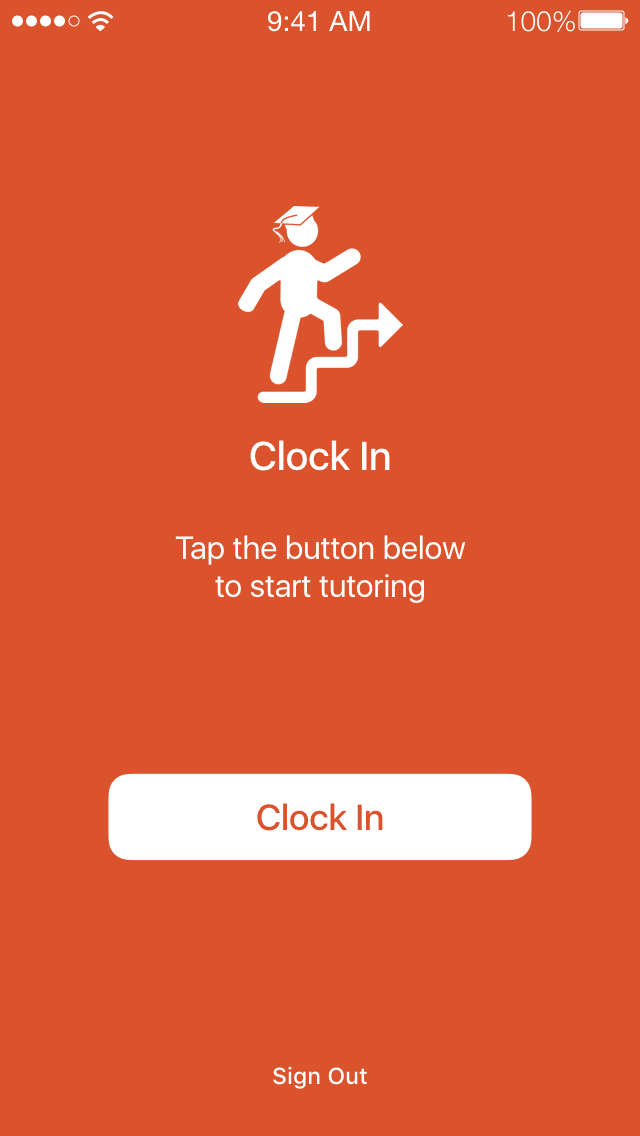
\includegraphics[scale=0.5]{e703e1125d.png}
\caption{Clock On}
\label{15}
\end{figure}



\begin{figure}[p]
\centering
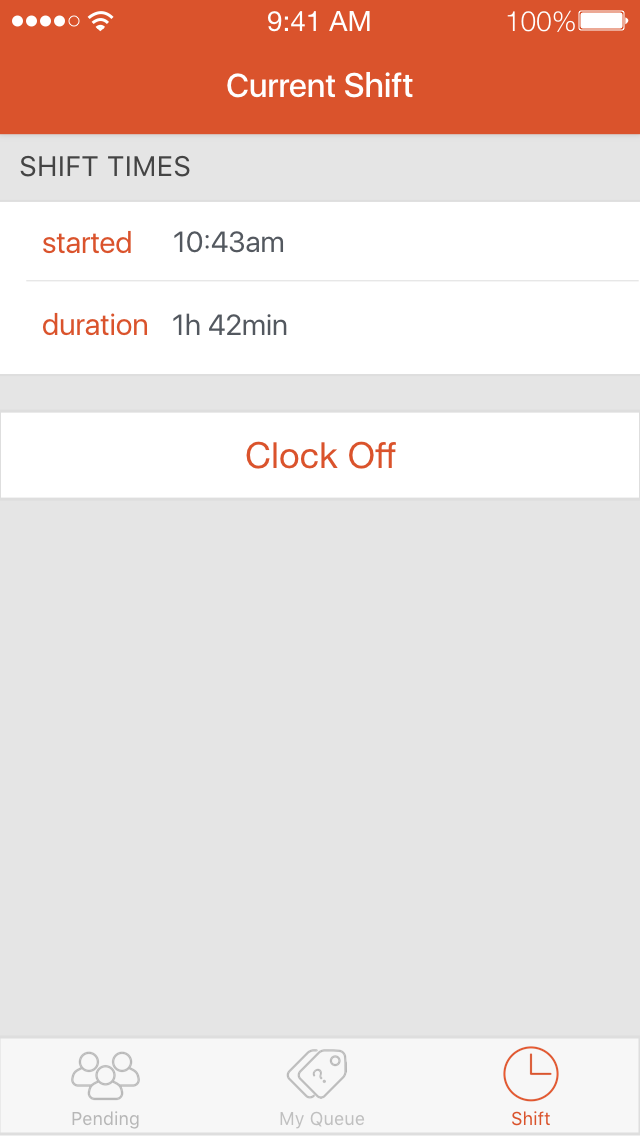
\includegraphics[scale=0.5]{5fe79d1e6c.png}
\caption{Shift Tab}
\label{16}
\end{figure}

\begin{figure}[p]
\centering
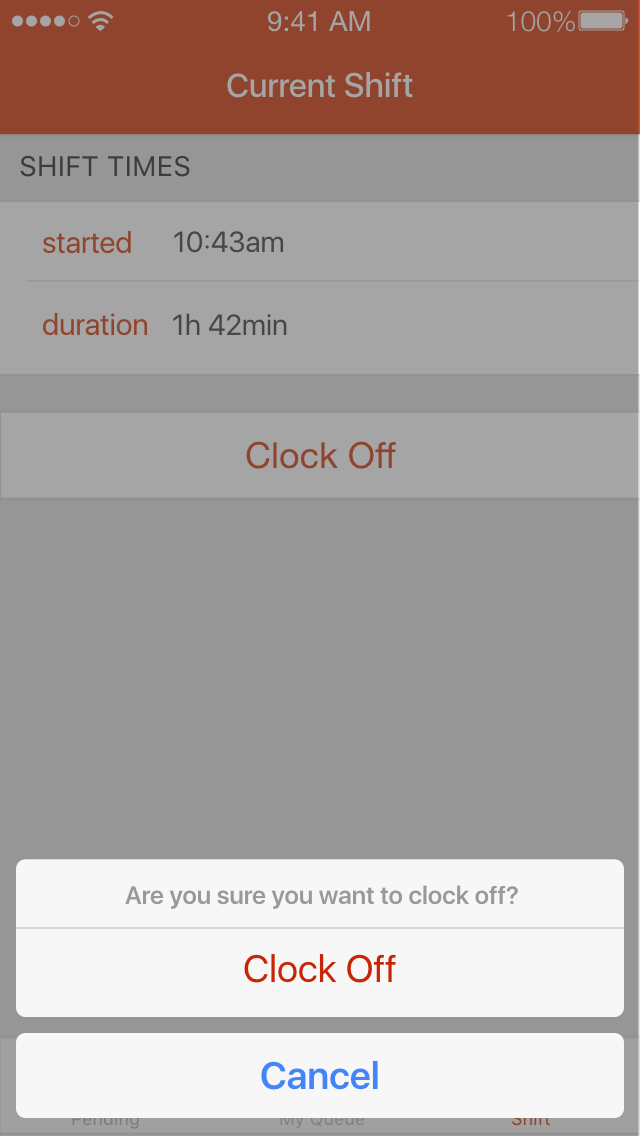
\includegraphics[scale=0.5]{2ac3c9eec5.png}
\caption{Shift Tab - Clocking Off}
\label{17}
\end{figure}


\end{document}
